\documentclass[
LEEC,			% Use this option to select your DEE degree, options: LEEC, LETI
english,		% Select document language, options: portuguese or english
%draft,	% Uncomment for draft mode (no pictures, no links, overfull hboxes) 
%twocolumn
]{DEEclass}

% Use the 'preamble.tex' file (root folder) do add packages and macros. Keep your main.tex file clean.

% FYI, the following packages are preloaded with the document class:
% longtable, xcolor, graphicx, booktabs, caption, csquotes, hyperref,
% calc, listings, datetime2, siunitx, geometry, enumitem

%%%%%%%%%%%%%%%%%%%%%%%%%%%%%%%%%%%%%%%%%%%%%%%%%%%%%%%%%% extra packages
\usepackage{amsmath}		% the main package in the AMS-LATEX distribution
\usepackage{amsfonts}		% extended set of fonts for use in mathematics
\usepackage{amssymb}		% adds new symbols to be used in math mode
\usepackage{mathrsfs}		% math fonts, e.g., Laplace
\usepackage{float}			% provides the H float modifier option
\usepackage{multirow}		% tables \multirow command
\usepackage{subcaption}		% enables subfigures
\usepackage{lscape}			% for landscape mode
\usepackage{verbatim}		% new verbatim environment, 
\usepackage{multicol}		% enables multicolumns 
\usepackage[intoc, english]{nomencl} % add nomenclature
\makenomenclature
\usepackage{etoolbox}       % used for nomenclature, i guess...
\makeglossaries
\usepackage{wrapfig}        % enable wrapping figures graphics
\usepackage{graphicx}       % enable graphics
\let\cleardoublepage=\clearpage     % delete blank pages
%\begin{comment}...\end{comment}, \verbatiminput


%add extra packages if needed here

%%%%%%%%%%%%%%%%%%%%%%%%%%%%%%%%%%%%%%%%%%%%%%%%%%%%%%%%%% temp packages
\usepackage{lipsum}						% for fake text
%\usepackage[textsize=tiny]{todonotes}   % enable To-do notes, use the option "disable" to hide all notes, usage \todo{}

%\usepackage{draftwatermark}			% prints a watermark overlay, uncomment if needed
%\SetWatermarkText{**DRAFT**}
%\SetWatermarkScale{1}
%\SetWatermarkColor[gray]{0.8}

%%%%%%%%%%%%%%%%%%%%%%%%%%%%%%%%%%%%%%%%%%%%%%%%%%%%%%%%%% settings
\AtBeginDocument{					% Rendered PDF metadata:
\hypersetup{pdftitle=\ttitle} 		% Sets the PDF title to your dissertation title
\hypersetup{pdfauthor=\authorname} 	% Sets the PDF author to your name
}

%%%%%%%%%%%%%%%%%%%%%%%%%%%%%%%%%%%%%%%%%%%%%%%%%%%%%%%%%% user defined macros









	
% \makenomenclature

%%%%%%%%%%%%%%%%%%%%%%%%%%%%%%%% REPORT INFORMATION %%%%%%%%%%%%%%%%%%%%%%%%%%%%%%%%%%%%%

\reporttitle{Example title} % Your report title

\author{Romain Lambert}	% Your name
\studentnumber{0673627662}	% Your student number
\studentemail{1234567@isep.ipp.pt}	% Your student email address  

\advisor{Nome do Orientador}{xxx@isep.ipp.pt}	% Your ISEP advisor name and email
\coadvisor{Nome do Coorientador}{xxx@isep.ipp.pt}	% Your ISEP co-advisor name and email, comment this line if not needed
\company{Nome da Empresa, Lda.}	% The company name where you developed your work, comment this line if not needed
\supervisor{Nome do Orientador da Empresa}{xxx@emailaddress.com} % Your company supervisor name, comment this line if not needed

%%%%%%%%%%%%%%%%%%%%%%%%%%%%%%%%%%%%%%%%%%%%%%%%%%%%%%%%%%%%%%%%%%%%%%%%%%%%%%%%%%%%%%%%%
\begin{document}

\pagestyle{plain} % Default to the plain heading style until the thesis style is called for the body content

\printcoverpage

%%%%%%%%%%%%%%%%%%%%%%%%%%%%%%%%%%% FRONTMATTER %%%%%%%%%%%%%%%%%%%%%%%%%%%%%%%%%%%%%%%%%
% Consider the following front matter sections provided as separate files in the 'front' folder.
% Comment the lines regarding the sections you will not use, or edit the file contents as needed

\tableofcontents

% \listoffigures
% %% This code creates the groups
% -----------------------------------------
\renewcommand\nomgroup[1]{%
  \item[\bfseries
  \ifstrequal{#1}{C}{Computational fluid dynamics}{%
  \ifstrequal{#1}{K}{Kite flight modelling}{%
  \ifstrequal{#1}{S}{Sailing vocabulary}{}}}%
]}
% -----------------------------------------

\nomenclature[C]{\(\textbf{CFD}\)}{Computational fluid dynamics}
\nomenclature[C]{\(\textbf{VLM}\)}{Vortex lattice method}

\nomenclature[k]{\(\textbf{V$_{WR}$}\)}{Relative wind velocity at kite altitude}
\nomenclature[k]{\(\textbf{V$_{WT}$}\)}{True wind velocity}
\nomenclature[k]{\(\textbf{V$_{s}$}\)}{Ship velocity}
\nomenclature[k]{\(\textbf{$\alpha_{i}$}\)}{Kite angle of attack}
\nomenclature[k]{\(\textbf{$\delta$}\)}{Angle between the athlete and his lines}
\nomenclature[k]{\(\textbf{V$_{a}$}\)}{Apparent wind velocity seen by the kite}
\nomenclature[k]{\(\textbf{V$_{k}$}\)}{Kite velocity}
\nomenclature[k]{\(\textbf{F$_{a}$}\)}{Aerodynamic resultant}
\nomenclature[k]{\(\textbf{T}\)}{Tethers tension}
\nomenclature[k]{\(\textbf{$\alpha_{S, WT}$}\)}{Angle between the rider and the true wind speed}
\nomenclature[k]{\(\textbf{$\epsilon$}\)}{Angle between the kite's velocity vector and the apparent wind}
\nomenclature[k]{\(\textbf{$\alpha_{a,WT}$}\)}{Angle between the apparent wind speed and the true wind speed}

\nomenclature[S]{\(\textbf{VMG}\)}{Velocity Made Good}
% \printnomenclature

%\include{front/2_acknowledgements}	% Edit to add the due acknowledgements, or comment this line if not used
%\include{front/3_abstract}			% Edit the file to write the document Abstract. Two languages are always required.
%\include{front/4_frontmatterlists}	% Edit the file to select the lists to be shown (figures, tables, source code segments, glossary, acronyms, symbols)

%%%%%%%%%%%%%%%%%%%%%%%%%%%%%%%%%%% MAINMATTER %%%%%%%%%%%%%%%%%%%%%%%%%%%%%%%%%%%%%%%%%

% Include the chapters of the document as separate files from the 'chapters' folder

%%%%%%%%%%%%%%%%%%%%%%%%%%%%%%%%%%%% Chapter Template

\chapter{2D steady simulations} 	% Main chapter title
\label{Chapter1} 		% For referencing the chapter elsewhere, usage \ref{Chapter1}

%%%%%%%%%%%%%%%%%%%%%%%%%%%%%%%%%%%%

The initial goal was to identify the factors that contribute to the VMG's superior efficiency compared to the R1V4 and make the necessary adjustments.

The first step involved identifying the parameters that respond to various flight conditions. Following that, a low-fidelity approach using XFLR5 was employed to compute the 2D aerodynamic coefficients, providing insights into the disparities between the airfoils. Subsequently, Fluent CFD software was utilized to obtain a more precise assessment of the aerodynamic coefficients for each airfoil during actual flight conditions.

This is a reference to an article \cite{example}.

%%%%%%%%%%%%%%%%%%%%%%%%%%%%%%%%%%%%%%%%%%%%%%%%%%%%%%%%%%%%%%%%%%%%%%%%%%%%%%%%
%%%%%%%%%%%%%%%%%%%%%%%%%%%%%%%%%%%% SECTION 1 %%%%%%%%%%%%%%%%%%%%%%%%%%%%%%%%%
%%%%%%%%%%%%%%%%%%%%%%%%%%%%%%%%%%%%%%%%%%%%%%%%%%%%%%%%%%%%%%%%%%%%%%%%%%%%%%%%

\section{Kite flight modelling}
\label{sec:Ch1.1}

Example
\begin{figure}[H]
    \centering
    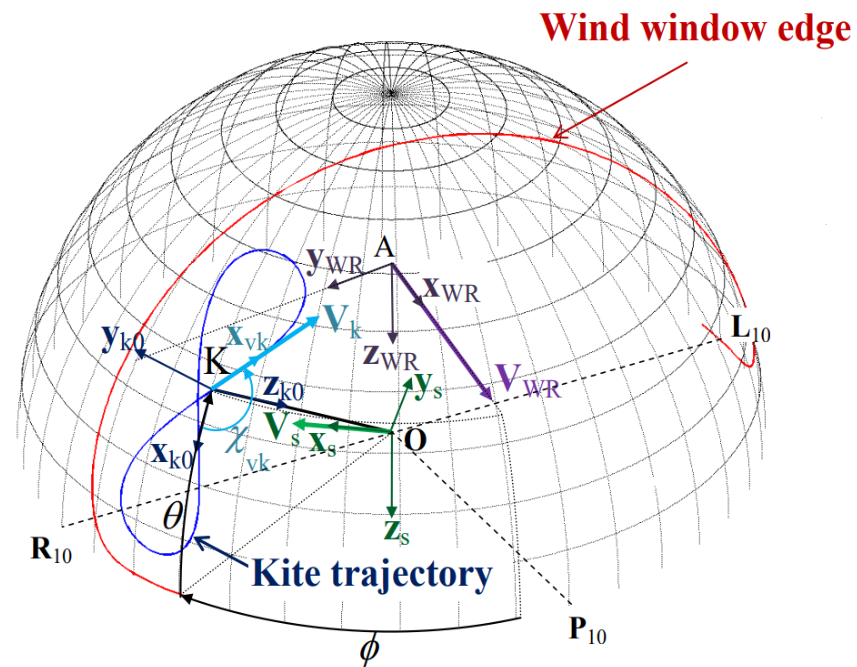
\includegraphics[width=0.7\textwidth]{figures/2D steady simulations/kite flight modeling 1.png}
    \caption{Speeds \& angles decomposition}
    \label{fig:Kite_flight_modelling}
\end{figure}


\begin{wrapfigure}{r}{0.6\textwidth}
\centering
    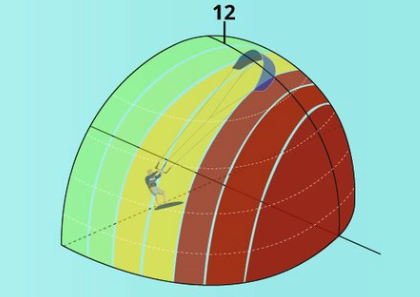
\includegraphics[width=0.5\textwidth]{figures/2D steady simulations/kite flight modeling 3.png}
    \caption{The wind window}
    \label{fig:The_wind_window}
\end{wrapfigure}

%%%%%%%%%%%%%%%%%%%%%%%%%%%%%%%%%%%%%%%%%%%%%%%%%%%%%%%%%%%%%%%%%%%%%%%%%%%%%%%%
%%%%%%%%%%%%%%%%%%%%%%%%%%%%%%%%%%%% SECTION 2 %%%%%%%%%%%%%%%%%%%%%%%%%%%%%%%%%
%%%%%%%%%%%%%%%%%%%%%%%%%%%%%%%%%%%%%%%%%%%%%%%%%%%%%%%%%%%%%%%%%%%%%%%%%%%%%%%%
\section{The different phases}
\label{sec:Ch1.3}

Example

%%%%%%%%%%%%%%%%%%%%%%%%%%%%%%%%%%%% SUBSECTION 1

\subsection{The upwind}
\label{sub:Ch1.3.1}

example
%%%%%%%%%%%%%%%%%%%%%%%%%%%%%%%%%%%% SUBSECTION 2

\subsection{The downwind}
\label{sub:Ch1.3.1}

Example

%%%%%%%%%%%%%%%%%%%%%%%%%%%%%%%%%%%%%%%%%%%%%%%%%%%%%%%%%%%%%%%%%%%%%%%%%%%%%%%%
%%%%%%%%%%%%%%%%%%%%%%%%%%%%%%%%%%%% SECTION 3 %%%%%%%%%%%%%%%%%%%%%%%%%%%%%%%%%
%%%%%%%%%%%%%%%%%%%%%%%%%%%%%%%%%%%%%%%%%%%%%%%%%%%%%%%%%%%%%%%%%%%%%%%%%%%%%%%%

\section{Experimental data }
\label{sec:Ch1.2}

\begin{table}[H]
    \center
    \begin{tabular}{|l|l|l|l|}
        \hline
            & $\alpha_{s, WT} ($°$) $ & $V_{WT} (knots) $ & $V_{S} (knots) $ \tabularnewline
        \hline
        Upwind & 39,5 & 14,0 & 22,5  \tabularnewline
        \hline
        Downwind & 155,0 & 14,0 & 31,5  \tabularnewline
        \hline
    \end{tabular}
    \caption{Average data from Axel's race}
    \label{tab:Average_data_from_Axels_race}
\end{table}
% Appendix A

\chapter{Título do Anexo} % Main appendix title
\label{AppendixA} % For referencing this appendix elsewhere, use \ref{AppendixA}

%%%%%%%%%%%%%%%%%%%%%%%%%%%%%%%%%%%%%%%%%%%%%%%%%%%%%%%%%%%%%%%%%%%%%%%%%%%%%%%%%%
\section{Secção}

Example

%%%%%%%%%%%%%%%%%%%%%%%%%%%%%%%%%%%%%%%%%%%%%%%%%%%%%%%%%%%%%%%%%%%%%%%%%%%%%%%%%%
\section{Mais uma secção do Anexo~\ref{AppendixA}}

Example





%%%%%%%%%%%%%%%%%%%%%%%%%%%%%%%%%%%%%%%%%%%%%%%%%%%%%%%%%%%%%%%%%%%%%%%%%%%%%%%%%%%%%%%%% BIBLIOGRAPHY

% Print the bibliographic references using the ieeetr format from the 'sampleRefs.bib' file (root folder)

% \clearpage

\addcontentsline{toc}{chapter}{References}
\bibliographystyle{plain} % We choose the "plain" reference style
\bibliography{references} % Entries are in the refs.bib file

								% a good option to make bib files is https://www.jabref.org/
			
%%%%%%%%%%%%%%%%%%%%%%%%%%%%%%%%%%%%%%%%%%%%%%%%%%%%%%%%%%%%%%%%%%%%%%%%%%%%%%%%%%%%%%%%% APPENDICES
%\begin{appendices}
% Include the appendices of the document as separate files from the 'chapters' folder

%% Appendix A

\chapter{Título do Anexo} % Main appendix title
\label{AppendixA} % For referencing this appendix elsewhere, use \ref{AppendixA}

%%%%%%%%%%%%%%%%%%%%%%%%%%%%%%%%%%%%%%%%%%%%%%%%%%%%%%%%%%%%%%%%%%%%%%%%%%%%%%%%%%
\section{Secção}

\lipsum[1]

%%%%%%%%%%%%%%%%%%%%%%%%%%%%%%%%%%%%%%%%%%%%%%%%%%%%%%%%%%%%%%%%%%%%%%%%%%%%%%%%%%
\section{Mais uma secção do Anexo~\ref{AppendixA}}

\lipsum[1]

	% Uncomment the lines as you write the appendices,
%\include{chapters/appendixB}	% or comment the lines if not used

%\end{appendices}
%%%%%%%%%%%%%%%%%%%%%%%%%%%%%%%%%%%%%%%%%%%%%%%%%%%%%%%%%%%%%%%%%%%%%%%%%%%%%%%%%%%%%%%%%
\end{document}  
